\section{Creating games and asking them questions}

Developing a prolog database that mirrors the conceptual model is not by itself useful. There need to be some functionality not present in the original model. Thus this implementation has two new functionalities: Possibility of describing a particular game, through its mechanics, dynamics and aesthetics, and thus creating a database of games. And the other is the availability of looking for suggestions to complete a game. 

\subsection{Game validity}

Defining a game in the program comes with the need of a predicate which verifies if a given game is valid. By valid we mean that all its components are in the model and that they interconnect through causal relationships. These requisites represent the MDA definition of what a game is. As this initial model is not comprehensive the value of creating this predicate is more indirect. A designer that wants to include his game in the database, use the predicate \textit{isGame()} including the mechanics his game have, and the dynamics and aesthetics identified through his play-testing experiences. If the predicate says the game is not valid it means either that there is no relationship between some of its concepts or have some component not present in the model. With this the user should consider improving the database with his experience, evaluating first if the components that are not in the model should to be included and most importantly where and how they must be. Then, considering the relationships between concepts, the user must evaluate by himself which causal relationships he observed in his playtesting and design and include them into the model.

Now that we have validity of games, it is possible to add games to the database without compromising it. To formalize this in the prolog program we define the predicate \textit{game} as:
\newline

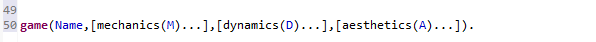
\includegraphics[]{Images/prologGame.png}

The first argument is a name for the game, aside from clarity it also allows for differentiation between games with the same components. The second, third and fourth arguments are lists. Each list should contain any number of atoms representing components of each type, respectively mechanics, dynamics and aesthetics. In other words the description of a game is his name with lists of components.

Verifying the validity of a game is made by a rule called \textit{isGame}. It is defined as:
\newline

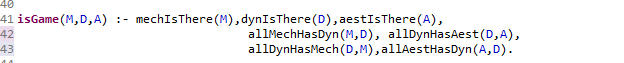
\includegraphics[]{Images/isGameprolog.png}
\newline

This rule checks every component list to make sure all elements are present in the database. Then it also verifies if there is a connection between each of its components. That is, each mechanic is connected to a dynamic and each dynamic is related to an aesthetic. Connected means either there is a relationship from mechanic to dynamic or there is a relationship from dynamic to mechanic. Negative results mean there is some error.

\subsection{Finding the error}

IsGame evaluates whether the game is valid, but in the negative case it does not point what is wrong with the description. Sometimes the user will want to find what makes a description incorrect. Manual investigation will be necessary to find this information. The first step should be to evaluate if every concept in the game description features in the model. Absent from the model, the user has to add the concept to the model or change its description to be in accordance with the model. How to deal with each of these situations is discussed in the next section.

Assured that all concepts of the description are part of the model, the next step is to check the relationships between the concepts. This is done by making sure that all components are connected, in other words, that no concept is isolated. To help the user in this investigation, some rules were created. Their objective is to evaluate possible representations inside the model structure. They do not specifically state what is incorrect. This is because they were create to fulfil other objectives discussed later. The first three are:

\begin{itemize}
    \item whatMech(D,A) : Prints a list of possible mechanics given a list of dynamics D and aesthetics A of the model. Possible means mechanics which have a valid relationship with the other concepts.
    \item whatDyn(M,A) : Prints a list of possible dynamics given a list of mechanics M and aesthetics A of the model. Possible means dynamics which have a valid relationship with the other concepts.
    \item whatAest(M,D) : Prints a list of possible aesthetics given a list of dynamics D and mechanics M of the model. Possible means aesthetics which have a valid relationship with the other concepts.
\end{itemize}

Summarizing, each rule displays all correct concepts of a type in respect to the given lists. With this the user can check if every concept of each part of his description is connected with at least one other type.

Assured that every concept of his list is included the model, the user now needs to evaluate the relationships. There is another set of rules that can improve this investigation. They aim to answer if there is a connection between two types of components in the user description. They are:

\begin{itemize}
    \item mechHasDyn(Mech,[D]) : checks if a given mechanic Mech is connected to at least one dynamic in list D.
    \item allMechHasDyn([M],[D]) : checks whether all mechanics in list M are connected to some dynamic in list D.
    
    \item aestHasDyn(Aest,[D]) : checks if a given aesthetic Aest is connected to at least one dynamic in list D.
    \item allAestHasDyn([A],[D]) : checks whether all aesthetics in list A are connected to some dynamic in list D.
    
    \item dynHasMech(Dyn,[M]) : checks if a given dynamic Dyn is connected to at least one mechanic in list M.
    \item allDynHasMech([D],[M]) : checks whether all dynamics in list D are connected to some dynamic in list M.
    
    \item dynHasAest(Dyn,[A]) : checks if a given dynamic Dyn is connected to at least one aesthetic in list A.
    \item allDynHasAest([D],[A]) : checks whether all dynamics in list D are connected to some aesthetic in list A.
    
\end{itemize}

Each combination of types can be investigated using these rules. For each pair there is one that verifies a single component against a list and another to compare two lists. Investigating thoroughly which component of your description is wrong will mainly use the comparisons of a single component. It will be able to pinpoint the incorrect part of the description. Given the four types of relationships present, finding which concept is wrong would take a considerable effort. The \textit{all} rules were created to quicken this task. They evaluate if the incorrectness is within a given relationship. Executing all four of them will tell the user where he does not need to investigate.

Capable now of evaluating the incorrectness of the description, the user is fully capable of utilizing the model to his own purposes. If he ever decide the model needs to be incremented, he should do it in accordance with the ideas discussed in the following section.